\documentclass[aps,prb,twocolumn,
	groupedaddress,superscriptaddress,
	amsfonts,amssymb,amsmath,floatfix,
	citeautoscript]{revtex4-1}

\usepackage{graphicx}
\usepackage[centering,hmargin=20mm,tmargin=30mm,bmargin=25mm]{geometry}
\usepackage{multirow}
\usepackage{newtxtext}
\usepackage[cmintegrals]{newtxmath}

%----- References -----
\usepackage{xcolor}
\usepackage{hyperref}
\hypersetup{colorlinks,
	linkcolor={blue!75!black!80!yellow},
	citecolor={blue!75!black!80!yellow},
	urlcolor={blue!75!black!80!yellow}
}

%----- Captions in sans font -----
\makeatletter
\renewcommand\@make@capt@title[2]{%
	\@ifx@empty\float@link{\@firstofone}{\expandafter\href\expandafter{\float@link}}%
	\sffamily{\textbf{#1}}\@caption@fignum@sep#2
}%
\renewcommand\figurename{Fig.}
\makeatother

\thickmuskip=5mu plus 2mu minus 1mu  %binary relations (default, 5mu plus 5mu)
\medmuskip=4mu plus 2mu minus 2mu    %binary operations (default, 4mu plus 2mu minus 4mu)

\frenchspacing %Ensure that revTeX does not do "double spaces" after punctuation

\renewcommand{\Im}{\operatorname{Im}}
\renewcommand{\Re}{\operatorname{Re}}
\newcommand{\sub}[1]{\ensuremath{_{\textrm{#1}}}} %Upright multi-character subscript
\newcommand{\super}[1]{\ensuremath{^{\textrm{#1}}}} %Upright multi-character superscript

\newcommand{\HarvardSEAS}{John A. Paulson School of Engineering and Applied Sciences, Harvard University, Cambridge, MA, USA}
\newcommand{\MITPhy}{Department of Physics, Massachusetts Institute of Technology, Cambridge, MA, USA}

%\usepackage[usenames]{color}
%\newcommand{\edited}[1]{{\color{red} #1}}

\begin{document}

\title{Variational theory of the ground state of quantum electrodynamics}

\author{Nicholas Rivera$^\perp$}\email{nrivera@seas.harvard.edu}\affiliation{\HarvardSEAS}\affiliation{\MITPhy}
\author{Johannes Flick}\email{flick@g.harvard.edu}\affiliation{\HarvardSEAS}
\author{Prineha Narang}\email{prineha@seas.harvard.edu}\affiliation{\HarvardSEAS}


\date{\today}

\begin{abstract}
In this work, we develop a variational theory of the ground state of a quantum electrodynamical system of coupled light and matter. Essential to our ansatz is the notion an effective photonic vacuum. As a first step towards an eventually \textit{ab initio} approach to ground states in QED, we apply our ansatz to a Rabi model involving a multi-level emitter with many optical modes, a model which cannot be analytically solved. We find a compact semi-analytic formula which describes the ground state energy very accurately in all regimes of coupling parameters.
\end{abstract}

\maketitle

The past decade has brought an explosion of effort and experimental progress in realizing the coupling of matter and quantized electromagnetic fields beyond a regime of weak coupling, in which perturbative treatments can accurately describe the dynamics. 

In what follows, we develop a variational ansatz for the ground state of quantum electrodynamical Hamiltonians. In particular, we develop an ansatz in which the ground state can be considered as a factorizable state of an effective matter and effective photon quasiparticle both in their respective ground states. This ansatz, analogous to the Hartree-Fock ansatz, leads to coupled eigen-equations describing the ground-state of the light-matter system. We benchmark our ansatz against a multi-level and multi-mode Rabi model parameterized by the strength of the characteristic momentum matrix elements describing the coupling of the matter and the electromagnetic fields. We find that when the momentum matrix elements are sufficiently weak, our theory finds the ground state energy to a remarkable accuracy of less than >99.9\%, even in the non-perturbative coupling regime. Even in regimes where the correlation energy is 50\% of the total energy, far outside of the validity domain of our ansatz, our ansatz predicts the energy up to a few percent. In regimes where our results are accurate, we claim we have found the effective quasiparticle description of the ground state. Moreover, in this regime, the ground state interaction energy manifests itself as the difference in zero-point energies between the quasiparticles and the bare particles. This generalizes the notion of the Casimir energy to a single atom in a cavity.

Our results service several aims. First, they suggest a novel variational approach for understanding ground states in ultra-strongly coupled light-matter systems. Second, they provide a general framework for understanding light-matter decoupling effects in the regime of strong light-matter interactions. Third, they prove a non-perturbative theory of Casimir-Polder forces. Finally, they provide a rigorous concept of correlation energy in quantum electrodynamics in a way analogous to electronic structure theory. 

The outline of this work is as follows: in section I, we develop the variational ansatz for the ground state of the Hamiltonian of macroscopic quantum electrodynamics. In section II, we calculate the ground state energy according to this ansatz for the multi-level and multi-mode Rabi model and compare it to numerical diagonalization of the same problem. In section III, we study the accuracy of our ansatz as a function of the correlation energy in the system, and test several approaches to recover the correlation energy.  We consider both perturbation theory formulated in the interacting modes as well as a self-consistent perturbation theory which allows the perturbative energy shift to influence the modes.


In this work, we consider the light-matter Hamiltonian corresponding to an emitter placed at position $z=d$ in a one-dimensional cavity oriented along the $z$-direction. As the cavity is considered for simplicity to be one-dimensional, the electric field is oriented along a single direction, denoted $x$, while the magnetic field is oriented along a direction transverse to both the electric field and the cavity length, denoted $y$. We consider the interaction in the velocity gauge. The Hamiltonian can then be written as:
\begin{equation}
H = H_{\text{matter}}+\frac{\epsilon_0}{2}\int dz~(E^2+c^2B^2)+\frac{e}{m}A(d)p + \frac{q^2}{2m}A^2(d).
\end{equation}
The fields can be expressed as a mode expansion via:
\begin{equation}
A(z,t) = \sum\limits_{n=1}^{\infty} \sqrt{\frac{\hbar}{2\epsilon_0\omega_n }}(F_n(z)a_ne^{-i\omega_n t}+F^*_n(z)a_n^{\dagger}e^{i\omega_n t}),
\end{equation}
with $E(z,t) = -\partial_t A(z,t)$ and $B(z,t)=\partial_z A(z,t)$.  The $F_n(z)$ are the mode functions of the cavity, normalized such that $\int dz ~|F_n(z)|^2 = 1$. For a cavity of length $L$ the modes are given by $F_n(z) = \sqrt{\frac{2}{L}}\sin\left(\frac{n\pi z}{L} \right)$ and the corresponding mode frequencies are $\omega_n = \frac{n\pi c}{L}$. The matter Hamiltonian we take to be a multilevel system with an arbitrary number of levels, $N_a$. The matter system we describe as an $N_a$ site system. This could be considered as a simple model of a molecule within a tight-binding description. Thus we parameterize the general family of matter Hamiltonians as:
\begin{equation}
H_{\text{matter}} = \sum\limits_{i=1}^{{N_a-1}} V_i|i\rangle\langle i|+t(|i\rangle\langle i+1|+|i+1\rangle\langle i|) 
\end{equation}
The momentum operator, we write in a finite-different representation as
\begin{equation}
p = \frac{i}{R}\sum\limits_{i=1}^{N_a-1} \left(|i\rangle\langle i+1|-|i+1\rangle\langle i| \right),
\end{equation}
where $R$ is a constant with units of length representing roughly the difference in positions between sites. This physical interpretation however is rough: it is also a function of the hopping elements $t$, because we choose $R$ in this work such that the following sum rule is enforced:
\begin{equation}
\frac{2}{m}\sum\limits_{i=2}^{N_a}\frac{|p_{ig}|^2}{E_i - E_a} = 1,
\end{equation}
which is the Thomas-Reiche-Kuhn sum rule. Of course, this sum rule does not rigorously apply to a discrete-level system. However, the matrix elements and energy levels of a few-level approximated Hamiltonian  are derived from an underlying real-space (infinite dimensional) Hamiltonian, a discrete system which has  $\frac{2}{m}\sum\limits_{i=2}^{N_a}\frac{|p_{ig}|^2}{E_i - E_a} > 1$ cannot. As we shall show later in the text however, it does place a bound on how strong the effect of the $Ap$ term can be on the total energy. The net effect is that the value of $R$ we choose is on the order of $\sqrt{\frac{\hbar}{2mt}}$.

\section{Variational ansatz}
\begin{figure*}[t]
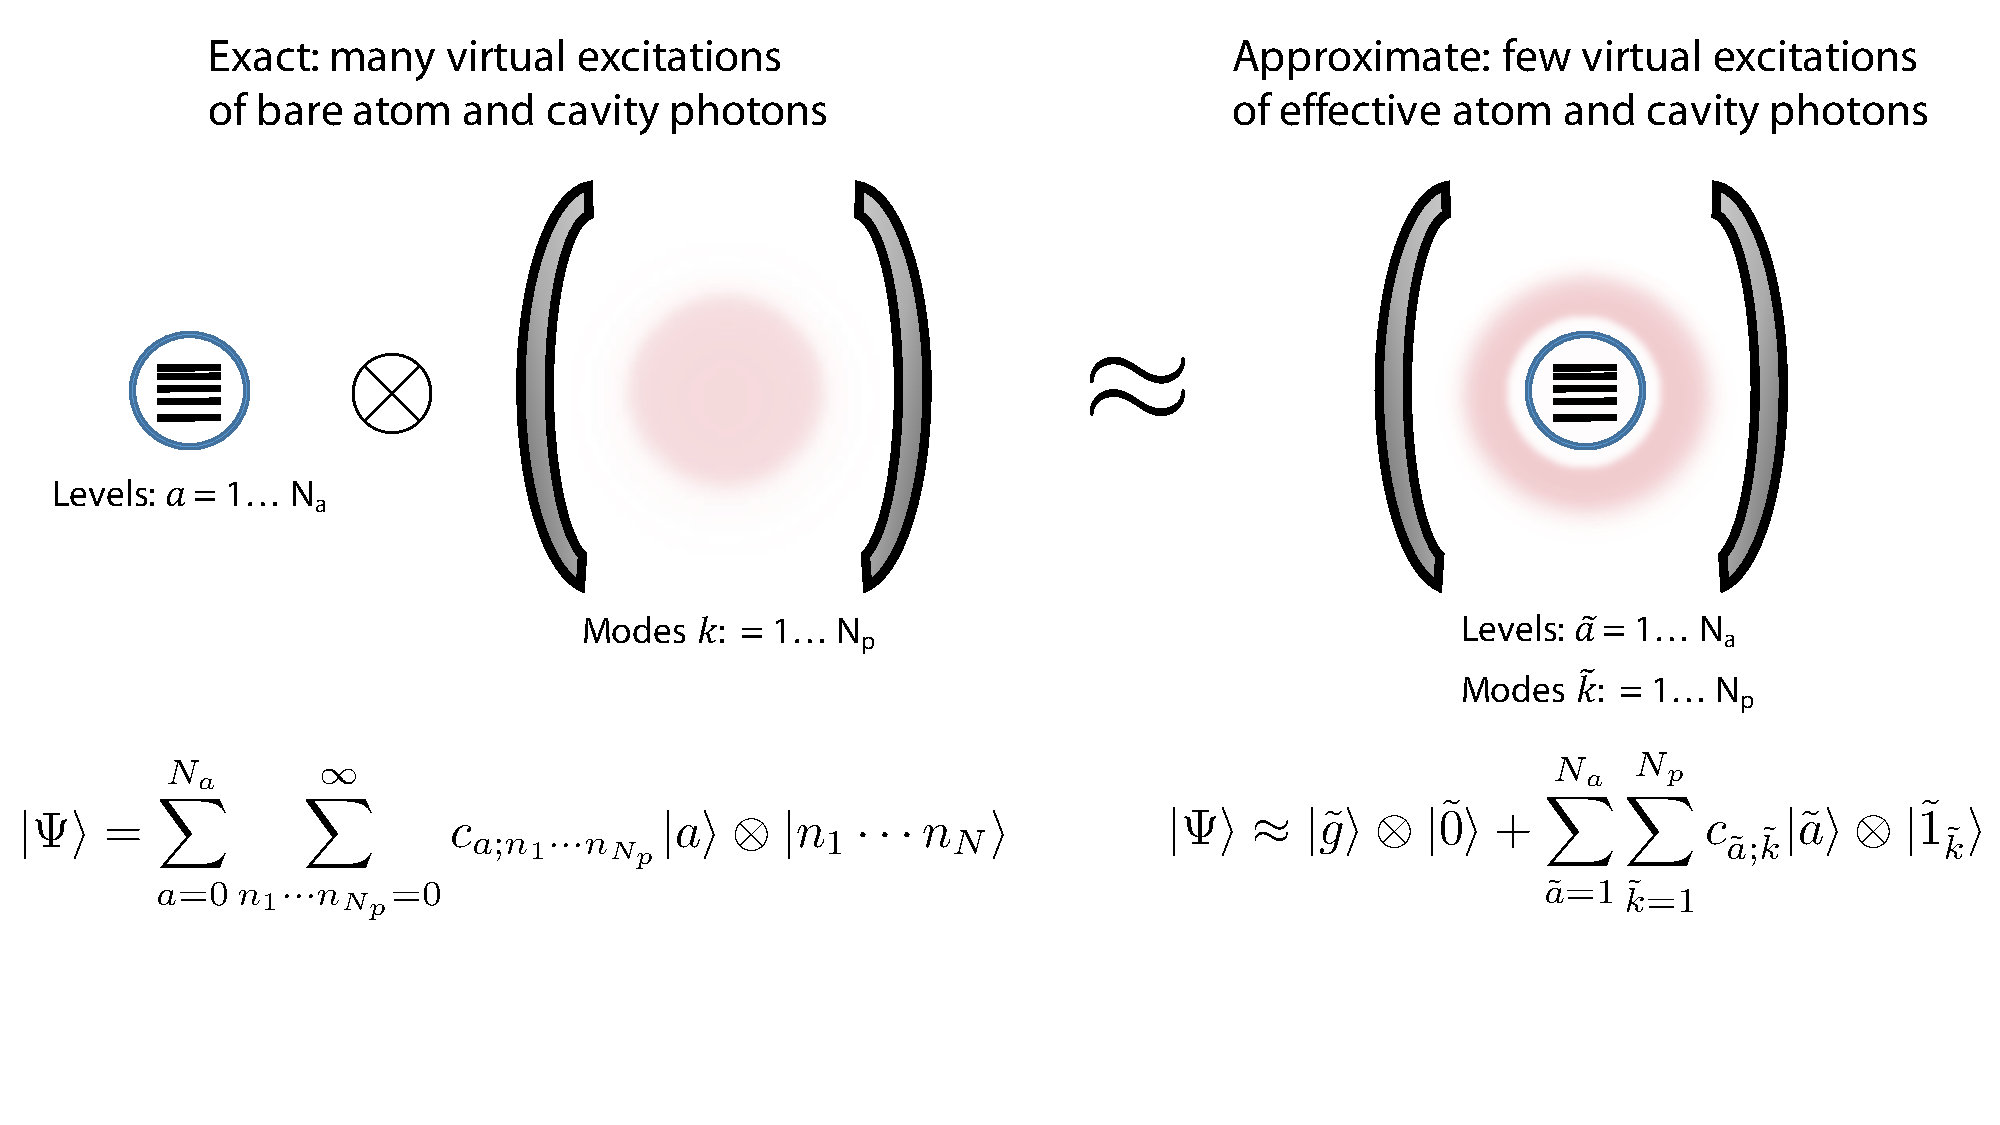
\includegraphics[width=16cm]{conceptfigure.pdf}
\caption{\textbf{Ground-state ansatz applied to matter in a cavity: effectively decoupled matter and photons.} (Left) Bare description of the coupled light-matter ground state in terms of many virtual excitations of the emitter state and the bare cavity photons. (Right) Quasiparticle description of the coupled system as a factorable state an effective emitter in its ground state and the vacuum of an effective photonic degree of freedom.}
\label{fig:ansatz}
\end{figure*}

The concept behind the variational ansatz is shown in Figure (1). We seek a description of the ground state of the system as $|\Psi\rangle \approx |\tilde{g}\rangle\otimes|\tilde{0}\rangle + |\delta\rangle,$ where a $\sim$ denotes an effective quantity. In other words, we seek a description in which the state is a factorizable state of matter and photon \textit{quasi}particles, up to some correlations quantified by the state $|\delta\rangle$. These correlations essentially hybridize $|\tilde{g}\rangle\otimes|\tilde{0}\rangle$ with excitations of the effective emitter and virtual effective photons. 

We start our analysis by considering a family of ansatze in which $\delta = 0$ (uncorrelated ansatz).  The expectation value of the Hamiltonian is 
\begin{align}
\langle \Psi | H | \Psi \rangle &= \langle \tilde{g} |H_{\text{matter}} | \tilde{g}\rangle \nonumber \\ &+ \frac{\hbar}{4}\int dz ~\sum\limits_{n=1}^{\infty}\left(\omega_n|F_n|^2 - \frac{c^2}{\omega_n}F_n^*\partial_z^2F_n\right) \nonumber \\ &+ \frac{\hbar q^2}{4m\epsilon_0\omega_n}\sum\limits_{n=1}^{\infty} \int dz~\delta(z-d)|F_n|^2
\end{align}
Notably, in this ansatz, the term in the Hamiltonian coupling the momentum of the matter to the photon makes no contribution. We impose constraints of matter normalization and photon mode normalization by defining a Lagrange function $\mathcal{L} \equiv \langle \Psi | H | \Psi \rangle - \epsilon(\langle \tilde{g}|\tilde{g}\rangle-1)-\sum\limits_{n=1}^{\infty}\frac{\hbar\lambda_n}{2}\left( \int dz~|F_n|^2-1\right)$. To find the ground state, we minimize the Lagrange function with respect to the matter orbital $|\tilde{g}\rangle$ and with respect to the mode functions $F_n$. The minimization with respect to the matter leads to the trivial equation $H_{\text{matter}} |\tilde{g}\rangle = \epsilon|\tilde{g}\rangle$ which leaves the effective matter ground state as simply the ground state of $H_{\text{matter}}$. On the other hand, the minimization with respect to the photon mode functions leads to  the equation
\begin{equation}
\left(\partial_z^2-\frac{\omega^2_n}{c^2}+2\frac{\omega_n\lambda_n}{c^2}-\frac{q^2 }{m\epsilon_0 c^2}\delta(z-d)\right)F_n  = 0.
\end{equation}
We may constrain $\lambda$ by differentiating the Lagrange function also with respect to the $\omega_n$. The equation which follows is:
\begin{equation}
\int dz ~\left(|F_n|^2 + \frac{c^2}{\omega^2_n}F_n^*\partial_z^2F_n\right) - \frac{ q^2}{m\epsilon_0\omega^2_n} \int dz~\delta(z-d)|F_n|^2 = 0
\end{equation}
Performing $\frac{\omega_n^2}{c^2}\int dz~F_n^*$ on both sides of Equation (5), and adding this equation to Equation (6), one immediately finds that $\lambda_n = \omega_n$ and that
\begin{equation}
\left(\partial_z^2+\frac{\omega^2_n}{c^2}-\frac{q^2 }{m\epsilon_0 c^2}\delta(z-d)\right)F_n  = 0.
\end{equation}

This is an ordinary second-order differential equation with the conditions that $F_n$ is continuous at $d$ and that its derivative is discontinuous according to 
\begin{equation}
\partial_zF_n\Big|_{z=d^+}-\partial_zF_n\Big|_{z=d^-} = \frac{q^2}{m\epsilon_0 c^2}F_n(d),
\end{equation}
in addition to the usual condition of the modes vanishing at the cavity walls $z=0$ and $z=L$. It can be shown that the solution to Equation (7) satisfying such boundary conditions is:
\begin{align}
&\theta (z-d) \left(\frac{\sin\left(\frac{\omega_nL}{c}\right)\sin\left(\frac{\omega_nd}{c}\right)\cos\left(\frac{\omega_nz}{c}\right)}{\sin\left(\frac{\omega_n(L-d)}{c}\right)}-\right) \nonumber \\ 
-&\theta (z-d) \left(\frac{\cos\left(\frac{\omega_nL}{c}\right)\sin\left(\frac{\omega_nd}{c}\right)\sin\left(\frac{\omega_nz}{c}\right)}{\sin\left(\frac{\omega_n(L-d)}{c}\right)}\right) \nonumber \\ 
+&\theta (d-z) \sin\left(\frac{\omega_n z}{c} \right)
\end{align}
provided that the auxiliary condition
\begin{equation}
\cot\left(\frac{\omega_n}{c}d \right)+\cot\left(\frac{\omega_n}{c}(L-d) \right) = \frac{q^2}{4m\epsilon_0\omega_nc}
\end{equation}
is met. To ensure that the modes are normalized according to the constraint, we have that the solutions of Equation (9) must be multiplied by a normalization factor $N_n$ given by
\begin{equation}
N_n = 2\sqrt{\frac{c}{\omega_n\left(\frac{\omega_nL}{c}-\sin\left(\frac{\omega_nL}{c}\right) \right)\left(1+\frac{\sin^2\left(\frac{\omega_nd}{c}\right)}{\sin^2\left(\frac{\omega_n(L-d)}{c}\right)} \right)}}.
\end{equation}
The condition of Equation (9) determines the resonance frequencies of the photon quasiparticle modes. After calculating the modes and the frequencies, we may move to an evaluation of the energy of the ground state. We proceed by taking the solutions of Equation (9), normalized with the normalization factor of Equation (11), and plugging it back into the expectation value of the Hamiltonian of the ground state (Equation (4)). After plugging in the quasiparticle photon modes into Equation (4), we find that
\begin{equation}
\langle \Psi | H|\Psi\rangle = E_{g}+\frac{1}{2}\sum\limits_{n=1}^{\infty}\hbar\omega_n.
\end{equation}
The interaction energy, which is the difference between the ground state energy with $q\neq 0$ and the non-interacting ground state energy, is $\frac{1}{2}\sum\limits_{n=1}^{\infty}\hbar(\omega_n-\omega_n^0)$, where $\omega_n^0 = \frac{n\pi c}{L}$ are the frequencies of the bare cavity modes. The result just derived establishes that the interaction energy within this ansatz is the Casimir energy of the system. This is quite interesting as typically when one calculates a Casimir energy, what is calculated is the zero-point energy associated with the electromagnetic modes of \textit{macroscopic polarizable objects}. Here on the other hand, we consider the \textit{electromagnetic modes of a single atom in a cavity}.

\section{Application to a multi-level system coupled to a multi-mode cavity}

%\section{Strategies for recovering the correlation energy}

\section{Outlook}



\section{Acknowledgements}
% Pri, Johannes: Please insert any other relevant acknowledgement information here!
We thank Joel Yuen-Zhou for useful discussions. N. R. recognizes the support of the DOE Computational Science Graduate Fellowship (CSGF) fellowship no.  DE-FG02-97ER25308. P. N. acknowledges start-up funding from the Harvard John A. Paulson School of Engineering and Applied Sciences. %The authors thank XXXX for helpful discussions. Tentatively Joel Yuen Zhou and Javier Aizpurua.

\bibliographystyle{apsrev4-1}
\bibliography{references}

\end{document}
